\documentclass[1p]{elsarticle_modified}
%\bibliographystyle{elsarticle-num}

%\usepackage[colorlinks]{hyperref}
%\usepackage{abbrmath_seonhwa} %\Abb, \Ascr, \Acal ,\Abf, \Afrak
\usepackage{amsfonts}
\usepackage{amssymb}
\usepackage{amsmath}
\usepackage{amsthm}
\usepackage{scalefnt}
\usepackage{amsbsy}
\usepackage{kotex}
\usepackage{caption}
\usepackage{subfig}
\usepackage{color}
\usepackage{graphicx}
\usepackage{xcolor} %% white, black, red, green, blue, cyan, magenta, yellow
\usepackage{float}
\usepackage{setspace}
\usepackage{hyperref}

\usepackage{tikz}
\usetikzlibrary{arrows}

\usepackage{multirow}
\usepackage{array} % fixed length table
\usepackage{hhline}

%%%%%%%%%%%%%%%%%%%%%
\makeatletter
\renewcommand*\env@matrix[1][\arraystretch]{%
	\edef\arraystretch{#1}%
	\hskip -\arraycolsep
	\let\@ifnextchar\new@ifnextchar
	\array{*\c@MaxMatrixCols c}}
\makeatother %https://tex.stackexchange.com/questions/14071/how-can-i-increase-the-line-spacing-in-a-matrix
%%%%%%%%%%%%%%%

\usepackage[normalem]{ulem}

\newcommand{\msout}[1]{\ifmmode\text{\sout{\ensuremath{#1}}}\else\sout{#1}\fi}
%SOURCE: \msout is \stkout macro in https://tex.stackexchange.com/questions/20609/strikeout-in-math-mode

\newcommand{\cancel}[1]{
	\ifmmode
	{\color{red}\msout{#1}}
	\else
	{\color{red}\sout{#1}}
	\fi
}

\newcommand{\add}[1]{
	{\color{blue}\uwave{#1}}
}

\newcommand{\replace}[2]{
	\ifmmode
	{\color{red}\msout{#1}}{\color{blue}\uwave{#2}}
	\else
	{\color{red}\sout{#1}}{\color{blue}\uwave{#2}}
	\fi
}

\newcommand{\Sol}{\mathcal{S}} %segment
\newcommand{\D}{D} %diagram
\newcommand{\A}{\mathcal{A}} %arc


%%%%%%%%%%%%%%%%%%%%%%%%%%%%%5 test

\def\sl{\operatorname{\textup{SL}}(2,\Cbb)}
\def\psl{\operatorname{\textup{PSL}}(2,\Cbb)}
\def\quan{\mkern 1mu \triangleright \mkern 1mu}

\theoremstyle{definition}
\newtheorem{thm}{Theorem}[section]
\newtheorem{prop}[thm]{Proposition}
\newtheorem{lem}[thm]{Lemma}
\newtheorem{ques}[thm]{Question}
\newtheorem{cor}[thm]{Corollary}
\newtheorem{defn}[thm]{Definition}
\newtheorem{exam}[thm]{Example}
\newtheorem{rmk}[thm]{Remark}
\newtheorem{alg}[thm]{Algorithm}

\newcommand{\I}{\sqrt{-1}}
\begin{document}

%\begin{frontmatter}
%
%\title{Boundary parabolic representations of knots up to 8 crossings}
%
%%% Group authors per affiliation:
%\author{Yunhi Cho} 
%\address{Department of Mathematics, University of Seoul, Seoul, Korea}
%\ead{yhcho@uos.ac.kr}
%
%
%\author{Seonhwa Kim} %\fnref{s_kim}}
%\address{Center for Geometry and Physics, Institute for Basic Science, Pohang, 37673, Korea}
%\ead{ryeona17@ibs.re.kr}
%
%\author{Hyuk Kim}
%\address{Department of Mathematical Sciences, Seoul National University, Seoul 08826, Korea}
%\ead{hyukkim@snu.ac.kr}
%
%\author{Seokbeom Yoon}
%\address{Department of Mathematical Sciences, Seoul National University, Seoul, 08826,  Korea}
%\ead{sbyoon15@snu.ac.kr}
%
%\begin{abstract}
%We find all boundary parabolic representation of knots up to 8 crossings.
%
%\end{abstract}
%\begin{keyword}
%    \MSC[2010] 57M25 
%\end{keyword}
%
%\end{frontmatter}

%\linenumbers
%\tableofcontents
%
\newcommand\colored[1]{\textcolor{white}{\rule[-0.35ex]{0.8em}{1.4ex}}\kern-0.8em\color{red} #1}%
%\newcommand\colored[1]{\textcolor{white}{ #1}\kern-2.17ex	\textcolor{white}{ #1}\kern-1.81ex	\textcolor{white}{ #1}\kern-2.15ex\color{red}#1	}

{\Large $\underline{12n_{0580}~(K12n_{0580})}$}

\setlength{\tabcolsep}{10pt}
\renewcommand{\arraystretch}{1.6}
\vspace{1cm}\begin{tabular}{m{100pt}>{\centering\arraybackslash}m{274pt}}
\multirow{5}{120pt}{
	\centering
	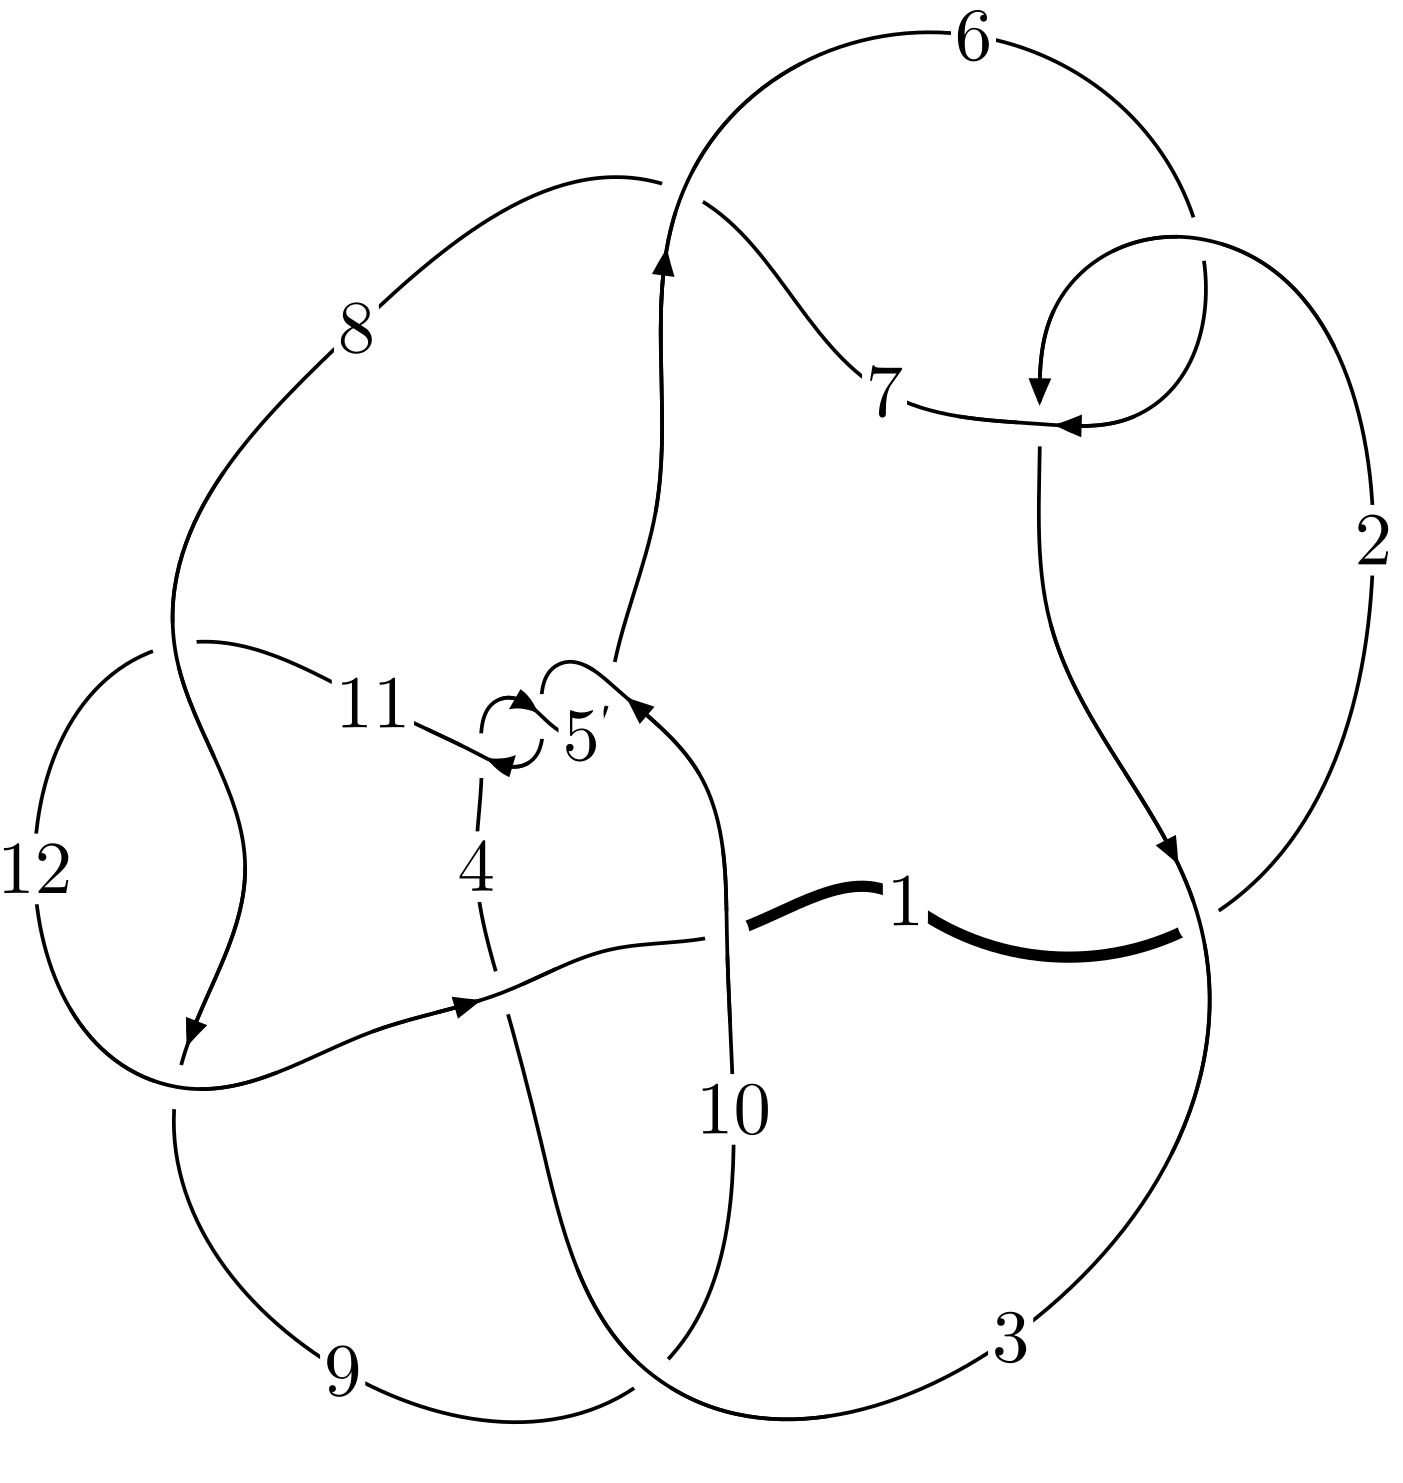
\includegraphics[width=112pt]{../../../GIT/diagram.site/Diagrams/png/2669_12n_0580.png}\\
\ \ \ A knot diagram\footnotemark}&
\allowdisplaybreaks
\textbf{Linearized knot diagam} \\
\cline{2-2}
 &
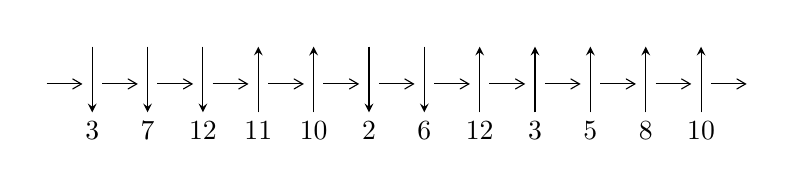
\begin{tikzpicture}[x=20pt, y=17pt]
	% nodes
	\node (C0) at (0, 0) {};
	\node (C1) at (1, 0) {};
	\node (C1U) at (1, +1) {};
	\node (C1D) at (1, -1) {3};

	\node (C2) at (2, 0) {};
	\node (C2U) at (2, +1) {};
	\node (C2D) at (2, -1) {7};

	\node (C3) at (3, 0) {};
	\node (C3U) at (3, +1) {};
	\node (C3D) at (3, -1) {12};

	\node (C4) at (4, 0) {};
	\node (C4U) at (4, +1) {};
	\node (C4D) at (4, -1) {11};

	\node (C5) at (5, 0) {};
	\node (C5U) at (5, +1) {};
	\node (C5D) at (5, -1) {10};

	\node (C6) at (6, 0) {};
	\node (C6U) at (6, +1) {};
	\node (C6D) at (6, -1) {2};

	\node (C7) at (7, 0) {};
	\node (C7U) at (7, +1) {};
	\node (C7D) at (7, -1) {6};

	\node (C8) at (8, 0) {};
	\node (C8U) at (8, +1) {};
	\node (C8D) at (8, -1) {12};

	\node (C9) at (9, 0) {};
	\node (C9U) at (9, +1) {};
	\node (C9D) at (9, -1) {3};

	\node (C10) at (10, 0) {};
	\node (C10U) at (10, +1) {};
	\node (C10D) at (10, -1) {5};

	\node (C11) at (11, 0) {};
	\node (C11U) at (11, +1) {};
	\node (C11D) at (11, -1) {8};

	\node (C12) at (12, 0) {};
	\node (C12U) at (12, +1) {};
	\node (C12D) at (12, -1) {10};
	\node (C13) at (13, 0) {};

	% arrows
	\draw[->,>={angle 60}]
	(C0) edge (C1) (C1) edge (C2) (C2) edge (C3) (C3) edge (C4) (C4) edge (C5) (C5) edge (C6) (C6) edge (C7) (C7) edge (C8) (C8) edge (C9) (C9) edge (C10) (C10) edge (C11) (C11) edge (C12) (C12) edge (C13) ;	\draw[->,>=stealth]
	(C1U) edge (C1D) (C2U) edge (C2D) (C3U) edge (C3D) (C4D) edge (C4U) (C5D) edge (C5U) (C6U) edge (C6D) (C7U) edge (C7D) (C8D) edge (C8U) (C9D) edge (C9U) (C10D) edge (C10U) (C11D) edge (C11U) (C12D) edge (C12U) ;
	\end{tikzpicture} \\
\hhline{~~} \\& 
\textbf{Solving Sequence} \\ \cline{2-2} 
 &
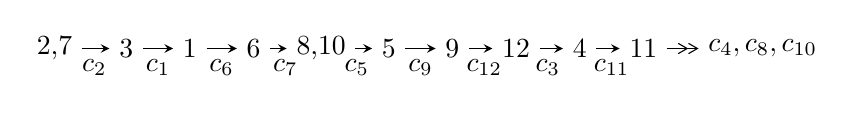
\begin{tikzpicture}[x=23pt, y=7pt]
	% node
	\node (A0) at (-1/8, 0) {2,7};
	\node (A1) at (1, 0) {3};
	\node (A2) at (2, 0) {1};
	\node (A3) at (3, 0) {6};
	\node (A4) at (65/16, 0) {8,10};
	\node (A5) at (41/8, 0) {5};
	\node (A6) at (49/8, 0) {9};
	\node (A7) at (57/8, 0) {12};
	\node (A8) at (65/8, 0) {4};
	\node (A9) at (73/8, 0) {11};
	\node (C1) at (1/2, -1) {$c_{2}$};
	\node (C2) at (3/2, -1) {$c_{1}$};
	\node (C3) at (5/2, -1) {$c_{6}$};
	\node (C4) at (7/2, -1) {$c_{7}$};
	\node (C5) at (37/8, -1) {$c_{5}$};
	\node (C6) at (45/8, -1) {$c_{9}$};
	\node (C7) at (53/8, -1) {$c_{12}$};
	\node (C8) at (61/8, -1) {$c_{3}$};
	\node (C9) at (69/8, -1) {$c_{11}$};
	\node (A10) at (11, 0) {$c_{4},c_{8},c_{10}$};

	% edge
	\draw[->,>=stealth]	
	(A0) edge (A1) (A1) edge (A2) (A2) edge (A3) (A3) edge (A4) (A4) edge (A5) (A5) edge (A6) (A6) edge (A7) (A7) edge (A8) (A8) edge (A9) ;
	\draw[->>,>={angle 60}]	
	(A9) edge (A10);
\end{tikzpicture} \\ 

\end{tabular} \\

\footnotetext{
The image of knot diagram is generated by the software ``\textbf{Draw programme}" developed by Andrew Bartholomew(\url{http://www.layer8.co.uk/maths/draw/index.htm\#Running-draw}), where we modified some parts for our purpose(\url{https://github.com/CATsTAILs/LinksPainter}).
}\phantom \\ \newline 
\centering \textbf{Ideals for irreducible components\footnotemark of $X_{\text{par}}$} 
 
\begin{align*}
I^u_{1}&=\langle 
-3 u^{20}+14 u^{19}+\cdots+2 b-4,\;- u^{20}+3 u^{19}+\cdots+2 a+3,\;u^{21}-6 u^{20}+\cdots+26 u-4\rangle \\
I^u_{2}&=\langle 
-463 u^5 a^3-277 u^5 a^2+\cdots-1475 a-789,\;- u^5 a^3-2 u^5 a^2+\cdots-2 a+6,\;u^6+u^5- u^4-2 u^3+u+1\rangle \\
I^u_{3}&=\langle 
- u^{11}+2 u^9- u^8-5 u^7+u^6+5 u^5-2 u^4-5 u^3+u^2+b+u,\\
\phantom{I^u_{3}}&\phantom{= \langle  }- u^{10}+2 u^8- u^7-5 u^6+u^5+5 u^4-2 u^3-5 u^2+a+u+1,\\
\phantom{I^u_{3}}&\phantom{= \langle  }u^{13}- u^{12}-2 u^{11}+3 u^{10}+4 u^9-6 u^8-4 u^7+8 u^6+3 u^5-7 u^4+3 u^2-1\rangle \\
\\
\end{align*}
\raggedright * 3 irreducible components of $\dim_{\mathbb{C}}=0$, with total 58 representations.\\
\footnotetext{All coefficients of polynomials are rational numbers. But the coefficients are sometimes approximated in decimal forms when there is not enough margin.}
\newpage
\renewcommand{\arraystretch}{1}
\centering \section*{I. $I^u_{1}= \langle -3 u^{20}+14 u^{19}+\cdots+2 b-4,\;- u^{20}+3 u^{19}+\cdots+2 a+3,\;u^{21}-6 u^{20}+\cdots+26 u-4 \rangle$}
\flushleft \textbf{(i) Arc colorings}\\
\begin{tabular}{m{7pt} m{180pt} m{7pt} m{180pt} }
\flushright $a_{2}=$&$\begin{pmatrix}1\\0\end{pmatrix}$ \\
\flushright $a_{7}=$&$\begin{pmatrix}0\\u\end{pmatrix}$ \\
\flushright $a_{3}=$&$\begin{pmatrix}1\\u^2\end{pmatrix}$ \\
\flushright $a_{1}=$&$\begin{pmatrix}- u^2+1\\- u^4\end{pmatrix}$ \\
\flushright $a_{6}=$&$\begin{pmatrix}u\\u\end{pmatrix}$ \\
\flushright $a_{8}=$&$\begin{pmatrix}- u^3\\- u^3+u\end{pmatrix}$ \\
\flushright $a_{10}=$&$\begin{pmatrix}\frac{1}{2} u^{20}-\frac{3}{2} u^{19}+\cdots+13 u-\frac{3}{2}\\\frac{3}{2} u^{20}-7 u^{19}+\cdots-\frac{29}{2} u+2\end{pmatrix}$ \\
\flushright $a_{5}=$&$\begin{pmatrix}-\frac{1}{4} u^{20}+3 u^{19}+\cdots+\frac{79}{4} u-4\\\frac{3}{2} u^{20}-5 u^{19}+\cdots+\frac{7}{2} u-1\end{pmatrix}$ \\
\flushright $a_{9}=$&$\begin{pmatrix}u^{20}-\frac{9}{2} u^{19}+\cdots-\frac{19}{2} u+\frac{5}{2}\\\frac{3}{2} u^{20}-6 u^{19}+\cdots-\frac{25}{2} u+2\end{pmatrix}$ \\
\flushright $a_{12}=$&$\begin{pmatrix}\frac{7}{4} u^{20}-7 u^{19}+\cdots-\frac{21}{4} u+2\\\frac{7}{2} u^{20}-16 u^{19}+\cdots-\frac{89}{2} u+7\end{pmatrix}$ \\
\flushright $a_{4}=$&$\begin{pmatrix}u^{20}-\frac{5}{2} u^{19}+\cdots+\frac{25}{2} u-\frac{3}{2}\\\frac{3}{2} u^{20}-6 u^{19}+\cdots-\frac{25}{2} u+2\end{pmatrix}$ \\
\flushright $a_{11}=$&$\begin{pmatrix}\frac{15}{4} u^{20}-14 u^{19}+\cdots+\frac{35}{4} u-2\\\frac{17}{2} u^{20}-40 u^{19}+\cdots-\frac{221}{2} u+17\end{pmatrix}$\\&\end{tabular}
\flushleft \textbf{(ii) Obstruction class $= -1$}\\~\\
\flushleft \textbf{(iii) Cusp Shapes $= -3 u^{20}+15 u^{19}-25 u^{18}-10 u^{17}+97 u^{16}-118 u^{15}-47 u^{14}+243 u^{13}-133 u^{12}-247 u^{11}+362 u^{10}+66 u^9-512 u^8+368 u^7+162 u^6-389 u^5+165 u^4+104 u^3-120 u^2+34 u+10$}\\~\\
\newpage\renewcommand{\arraystretch}{1}
\flushleft \textbf{(iv) u-Polynomials at the component}\newline \\
\begin{tabular}{m{50pt}|m{274pt}}
Crossings & \hspace{64pt}u-Polynomials at each crossing \\
\hline $$\begin{aligned}c_{1},c_{7}\end{aligned}$$&$\begin{aligned}
&u^{21}+8 u^{20}+\cdots+188 u+16
\end{aligned}$\\
\hline $$\begin{aligned}c_{2},c_{6}\end{aligned}$$&$\begin{aligned}
&u^{21}-6 u^{20}+\cdots+26 u-4
\end{aligned}$\\
\hline $$\begin{aligned}c_{3}\end{aligned}$$&$\begin{aligned}
&u^{21}-2 u^{20}+\cdots+5 u-1
\end{aligned}$\\
\hline $$\begin{aligned}c_{4},c_{5},c_{9}\\c_{10}\end{aligned}$$&$\begin{aligned}
&u^{21}+13 u^{19}+\cdots+u-1
\end{aligned}$\\
\hline $$\begin{aligned}c_{8},c_{11}\end{aligned}$$&$\begin{aligned}
&u^{21}-16 u^{20}+\cdots+480 u-64
\end{aligned}$\\
\hline $$\begin{aligned}c_{12}\end{aligned}$$&$\begin{aligned}
&u^{21}-3 u^{20}+\cdots-11 u-1
\end{aligned}$\\
\hline
\end{tabular}\\~\\
\newpage\renewcommand{\arraystretch}{1}
\flushleft \textbf{(v) Riley Polynomials at the component}\newline \\
\begin{tabular}{m{50pt}|m{274pt}}
Crossings & \hspace{64pt}Riley Polynomials at each crossing \\
\hline $$\begin{aligned}c_{1},c_{7}\end{aligned}$$&$\begin{aligned}
&y^{21}+12 y^{20}+\cdots+9072 y-256
\end{aligned}$\\
\hline $$\begin{aligned}c_{2},c_{6}\end{aligned}$$&$\begin{aligned}
&y^{21}-8 y^{20}+\cdots+188 y-16
\end{aligned}$\\
\hline $$\begin{aligned}c_{3}\end{aligned}$$&$\begin{aligned}
&y^{21}-36 y^{20}+\cdots+47 y-1
\end{aligned}$\\
\hline $$\begin{aligned}c_{4},c_{5},c_{9}\\c_{10}\end{aligned}$$&$\begin{aligned}
&y^{21}+26 y^{20}+\cdots- y-1
\end{aligned}$\\
\hline $$\begin{aligned}c_{8},c_{11}\end{aligned}$$&$\begin{aligned}
&y^{21}-6 y^{20}+\cdots-7168 y-4096
\end{aligned}$\\
\hline $$\begin{aligned}c_{12}\end{aligned}$$&$\begin{aligned}
&y^{21}+33 y^{20}+\cdots+43 y-1
\end{aligned}$\\
\hline
\end{tabular}\\~\\
\newpage\flushleft \textbf{(vi) Complex Volumes and Cusp Shapes}
$$\begin{array}{c|c|c}  
\text{Solutions to }I^u_{1}& \I (\text{vol} + \sqrt{-1}CS) & \text{Cusp shape}\\
 \hline 
\begin{aligned}
u &= \phantom{-}0.935175 + 0.517534 I \\
a &= -1.110460 - 0.861684 I \\
b &= -0.59252 - 1.38052 I\end{aligned}
 & \phantom{-}0.24926 - 3.91469 I & \phantom{-}2.72764 + 7.21725 I \\ \hline\begin{aligned}
u &= \phantom{-}0.935175 - 0.517534 I \\
a &= -1.110460 + 0.861684 I \\
b &= -0.59252 + 1.38052 I\end{aligned}
 & \phantom{-}0.24926 + 3.91469 I & \phantom{-}2.72764 - 7.21725 I \\ \hline\begin{aligned}
u &= \phantom{-}0.448329 + 0.989827 I \\
a &= -0.363224 - 1.287660 I \\
b &= \phantom{-}1.11171 - 0.93682 I\end{aligned}
 & -10.43170 + 7.68453 I & -0.20664 - 3.05097 I \\ \hline\begin{aligned}
u &= \phantom{-}0.448329 - 0.989827 I \\
a &= -0.363224 + 1.287660 I \\
b &= \phantom{-}1.11171 + 0.93682 I\end{aligned}
 & -10.43170 - 7.68453 I & -0.20664 + 3.05097 I \\ \hline\begin{aligned}
u &= \phantom{-}0.528861 + 1.017090 I \\
a &= -0.085943 + 1.202340 I \\
b &= -1.268340 + 0.548462 I\end{aligned}
 & -9.86050 - 1.84914 I & -0.90690 + 1.69467 I \\ \hline\begin{aligned}
u &= \phantom{-}0.528861 - 1.017090 I \\
a &= -0.085943 - 1.202340 I \\
b &= -1.268340 - 0.548462 I\end{aligned}
 & -9.86050 + 1.84914 I & -0.90690 - 1.69467 I \\ \hline\begin{aligned}
u &= -0.821760 + 0.209360 I \\
a &= \phantom{-}0.270782 - 0.182803 I \\
b &= -0.184246 + 0.206911 I\end{aligned}
 & -1.40817 + 0.64438 I & -3.79274 - 1.22685 I \\ \hline\begin{aligned}
u &= -0.821760 - 0.209360 I \\
a &= \phantom{-}0.270782 + 0.182803 I \\
b &= -0.184246 - 0.206911 I\end{aligned}
 & -1.40817 - 0.64438 I & -3.79274 + 1.22685 I \\ \hline\begin{aligned}
u &= -0.896473 + 0.746587 I \\
a &= -0.309151 + 0.124372 I \\
b &= \phantom{-}0.184291 - 0.342305 I\end{aligned}
 & \phantom{-}4.28731 + 2.84851 I & \phantom{-}0.39482 - 1.73871 I \\ \hline\begin{aligned}
u &= -0.896473 - 0.746587 I \\
a &= -0.309151 - 0.124372 I \\
b &= \phantom{-}0.184291 + 0.342305 I\end{aligned}
 & \phantom{-}4.28731 - 2.84851 I & \phantom{-}0.39482 + 1.73871 I\\
 \hline 
 \end{array}$$\newpage$$\begin{array}{c|c|c}  
\text{Solutions to }I^u_{1}& \I (\text{vol} + \sqrt{-1}CS) & \text{Cusp shape}\\
 \hline 
\begin{aligned}
u &= \phantom{-}0.677418 + 0.397216 I \\
a &= \phantom{-}1.51417 + 0.36850 I \\
b &= \phantom{-}0.879349 + 0.851081 I\end{aligned}
 & \phantom{-}1.096940 - 0.102856 I & \phantom{-}7.06481 + 1.59045 I \\ \hline\begin{aligned}
u &= \phantom{-}0.677418 - 0.397216 I \\
a &= \phantom{-}1.51417 - 0.36850 I \\
b &= \phantom{-}0.879349 - 0.851081 I\end{aligned}
 & \phantom{-}1.096940 + 0.102856 I & \phantom{-}7.06481 - 1.59045 I \\ \hline\begin{aligned}
u &= \phantom{-}0.904796 + 0.829662 I \\
a &= \phantom{-}0.401041 - 0.496617 I \\
b &= \phantom{-}0.774885 - 0.116608 I\end{aligned}
 & \phantom{-}4.71470 - 3.09578 I & -3.27109 + 3.56536 I \\ \hline\begin{aligned}
u &= \phantom{-}0.904796 - 0.829662 I \\
a &= \phantom{-}0.401041 + 0.496617 I \\
b &= \phantom{-}0.774885 + 0.116608 I\end{aligned}
 & \phantom{-}4.71470 + 3.09578 I & -3.27109 - 3.56536 I \\ \hline\begin{aligned}
u &= -1.327590 + 0.030849 I \\
a &= -0.070884 + 0.549935 I \\
b &= \phantom{-}0.077139 - 0.732274 I\end{aligned}
 & -17.1548 - 4.6029 I & -4.70163 + 2.09700 I \\ \hline\begin{aligned}
u &= -1.327590 - 0.030849 I \\
a &= -0.070884 - 0.549935 I \\
b &= \phantom{-}0.077139 + 0.732274 I\end{aligned}
 & -17.1548 + 4.6029 I & -4.70163 - 2.09700 I \\ \hline\begin{aligned}
u &= \phantom{-}1.176180 + 0.678965 I \\
a &= \phantom{-}1.80081 - 0.07045 I \\
b &= \phantom{-}2.16591 + 1.13982 I\end{aligned}
 & -12.7012 - 13.7507 I & -1.99835 + 6.85375 I \\ \hline\begin{aligned}
u &= \phantom{-}1.176180 - 0.678965 I \\
a &= \phantom{-}1.80081 + 0.07045 I \\
b &= \phantom{-}2.16591 - 1.13982 I\end{aligned}
 & -12.7012 + 13.7507 I & -1.99835 - 6.85375 I \\ \hline\begin{aligned}
u &= \phantom{-}1.175240 + 0.726178 I \\
a &= -1.45480 + 0.41477 I \\
b &= -2.01093 - 0.56899 I\end{aligned}
 & -11.89320 - 4.50624 I & -2.44659 + 2.53964 I \\ \hline\begin{aligned}
u &= \phantom{-}1.175240 - 0.726178 I \\
a &= -1.45480 - 0.41477 I \\
b &= -2.01093 + 0.56899 I\end{aligned}
 & -11.89320 + 4.50624 I & -2.44659 - 2.53964 I\\
 \hline 
 \end{array}$$\newpage$$\begin{array}{c|c|c}  
\text{Solutions to }I^u_{1}& \I (\text{vol} + \sqrt{-1}CS) & \text{Cusp shape}\\
 \hline 
\begin{aligned}
u &= \phantom{-}0.399649\phantom{ +0.000000I} \\
a &= \phantom{-}1.81531\phantom{ +0.000000I} \\
b &= \phantom{-}0.725488\phantom{ +0.000000I}\end{aligned}
 & \phantom{-}0.927006\phantom{ +0.000000I} & \phantom{-}12.2730\phantom{ +0.000000I}\\
 \hline 
 \end{array}$$\newpage\newpage\renewcommand{\arraystretch}{1}
\centering \section*{II. $I^u_{2}= \langle -463 u^5 a^3-277 u^5 a^2+\cdots-1475 a-789,\;- u^5 a^3-2 u^5 a^2+\cdots-2 a+6,\;u^6+u^5- u^4-2 u^3+u+1 \rangle$}
\flushleft \textbf{(i) Arc colorings}\\
\begin{tabular}{m{7pt} m{180pt} m{7pt} m{180pt} }
\flushright $a_{2}=$&$\begin{pmatrix}1\\0\end{pmatrix}$ \\
\flushright $a_{7}=$&$\begin{pmatrix}0\\u\end{pmatrix}$ \\
\flushright $a_{3}=$&$\begin{pmatrix}1\\u^2\end{pmatrix}$ \\
\flushright $a_{1}=$&$\begin{pmatrix}- u^2+1\\- u^4\end{pmatrix}$ \\
\flushright $a_{6}=$&$\begin{pmatrix}u\\u\end{pmatrix}$ \\
\flushright $a_{8}=$&$\begin{pmatrix}- u^3\\- u^3+u\end{pmatrix}$ \\
\flushright $a_{10}=$&$\begin{pmatrix}a\\0.246670 a^{3} u^{5}+0.147576 a^{2} u^{5}+\cdots+0.785828 a+0.420352\end{pmatrix}$ \\
\flushright $a_{5}=$&$\begin{pmatrix}-0.161961 a^{3} u^{5}-0.461907 a^{2} u^{5}+\cdots-0.777304 a-0.0340970\\-0.621204 a^{3} u^{5}-1.02824 a^{2} u^{5}+\cdots+0.604156 a-1.49920\end{pmatrix}$ \\
\flushright $a_{9}=$&$\begin{pmatrix}-0.246670 a^{3} u^{5}-0.147576 a^{2} u^{5}+\cdots+0.214172 a-0.420352\\-0.0223761 a^{3} u^{5}-0.728290 a^{2} u^{5}+\cdots+1.28077 a+0.784763\end{pmatrix}$ \\
\flushright $a_{12}=$&$\begin{pmatrix}-0.247736 a^{3} u^{5}-0.420352 a^{2} u^{5}+\cdots+0.465637 a+0.474161\\-0.656367 a^{3} u^{5}-0.0298348 a^{2} u^{5}+\cdots-0.0974960 a-2.98029\end{pmatrix}$ \\
\flushright $a_{4}=$&$\begin{pmatrix}0.134790 a^{3} u^{5}+0.506127 a^{2} u^{5}+\cdots+0.189664 a+1.34417\\1.31700 a^{3} u^{5}-0.849227 a^{2} u^{5}+\cdots+1.18913 a+5.38253\end{pmatrix}$ \\
\flushright $a_{11}=$&$\begin{pmatrix}-0.228556 a^{3} u^{5}-0.510389 a^{2} u^{5}+\cdots-0.0607352 a+0.372936\\-0.983484 a^{3} u^{5}-0.771977 a^{2} u^{5}+\cdots+0.102291 a-3.36494\end{pmatrix}$\\&\end{tabular}
\flushleft \textbf{(ii) Obstruction class $= -1$}\\~\\
\flushleft \textbf{(iii) Cusp Shapes $= \frac{808}{1877} u^5 a^3+\frac{4132}{1877} u^5 a^2+\cdots-\frac{2988}{1877} a-\frac{6350}{1877}$}\\~\\
\newpage\renewcommand{\arraystretch}{1}
\flushleft \textbf{(iv) u-Polynomials at the component}\newline \\
\begin{tabular}{m{50pt}|m{274pt}}
Crossings & \hspace{64pt}u-Polynomials at each crossing \\
\hline $$\begin{aligned}c_{1},c_{7}\end{aligned}$$&$\begin{aligned}
&(u^6+3 u^5+5 u^4+4 u^3+2 u^2+u+1)^4
\end{aligned}$\\
\hline $$\begin{aligned}c_{2},c_{6}\end{aligned}$$&$\begin{aligned}
&(u^6+u^5- u^4-2 u^3+u+1)^4
\end{aligned}$\\
\hline $$\begin{aligned}c_{3}\end{aligned}$$&$\begin{aligned}
&u^{24}-3 u^{23}+\cdots+54 u+43
\end{aligned}$\\
\hline $$\begin{aligned}c_{4},c_{5},c_{9}\\c_{10}\end{aligned}$$&$\begin{aligned}
&u^{24}- u^{23}+\cdots+148 u+43
\end{aligned}$\\
\hline $$\begin{aligned}c_{8},c_{11}\end{aligned}$$&$\begin{aligned}
&(u^2+u+1)^{12}
\end{aligned}$\\
\hline $$\begin{aligned}c_{12}\end{aligned}$$&$\begin{aligned}
&u^{24}+9 u^{23}+\cdots+376 u+229
\end{aligned}$\\
\hline
\end{tabular}\\~\\
\newpage\renewcommand{\arraystretch}{1}
\flushleft \textbf{(v) Riley Polynomials at the component}\newline \\
\begin{tabular}{m{50pt}|m{274pt}}
Crossings & \hspace{64pt}Riley Polynomials at each crossing \\
\hline $$\begin{aligned}c_{1},c_{7}\end{aligned}$$&$\begin{aligned}
&(y^6+y^5+5 y^4+6 y^2+3 y+1)^4
\end{aligned}$\\
\hline $$\begin{aligned}c_{2},c_{6}\end{aligned}$$&$\begin{aligned}
&(y^6-3 y^5+5 y^4-4 y^3+2 y^2- y+1)^4
\end{aligned}$\\
\hline $$\begin{aligned}c_{3}\end{aligned}$$&$\begin{aligned}
&y^{24}-33 y^{23}+\cdots-52280 y+1849
\end{aligned}$\\
\hline $$\begin{aligned}c_{4},c_{5},c_{9}\\c_{10}\end{aligned}$$&$\begin{aligned}
&y^{24}+27 y^{23}+\cdots+36576 y+1849
\end{aligned}$\\
\hline $$\begin{aligned}c_{8},c_{11}\end{aligned}$$&$\begin{aligned}
&(y^2+y+1)^{12}
\end{aligned}$\\
\hline $$\begin{aligned}c_{12}\end{aligned}$$&$\begin{aligned}
&y^{24}+27 y^{23}+\cdots+65640 y+52441
\end{aligned}$\\
\hline
\end{tabular}\\~\\
\newpage\flushleft \textbf{(vi) Complex Volumes and Cusp Shapes}
$$\begin{array}{c|c|c}  
\text{Solutions to }I^u_{2}& \I (\text{vol} + \sqrt{-1}CS) & \text{Cusp shape}\\
 \hline 
\begin{aligned}
u &= \phantom{-}1.002190 + 0.295542 I \\
a &= -1.050380 + 0.369608 I \\
b &= -1.20802 - 1.30034 I\end{aligned}
 & -6.82541 - 2.95419 I & -5.71672 + 4.25833 I \\ \hline\begin{aligned}
u &= \phantom{-}1.002190 + 0.295542 I \\
a &= -0.081771 + 0.727533 I \\
b &= \phantom{-}0.40776 + 1.96764 I\end{aligned}
 & -6.82541 + 1.10558 I & -5.71672 - 2.66988 I \\ \hline\begin{aligned}
u &= \phantom{-}1.002190 + 0.295542 I \\
a &= -1.46095 - 0.86667 I \\
b &= -1.161920 + 0.059986 I\end{aligned}
 & -6.82541 - 2.95419 I & -5.71672 + 4.25833 I \\ \hline\begin{aligned}
u &= \phantom{-}1.002190 + 0.295542 I \\
a &= \phantom{-}0.90697 + 1.69587 I \\
b &= -0.296966 + 0.704962 I\end{aligned}
 & -6.82541 + 1.10558 I & -5.71672 - 2.66988 I \\ \hline\begin{aligned}
u &= \phantom{-}1.002190 - 0.295542 I \\
a &= -1.050380 - 0.369608 I \\
b &= -1.20802 + 1.30034 I\end{aligned}
 & -6.82541 + 2.95419 I & -5.71672 - 4.25833 I \\ \hline\begin{aligned}
u &= \phantom{-}1.002190 - 0.295542 I \\
a &= -0.081771 - 0.727533 I \\
b &= \phantom{-}0.40776 - 1.96764 I\end{aligned}
 & -6.82541 - 1.10558 I & -5.71672 + 2.66988 I \\ \hline\begin{aligned}
u &= \phantom{-}1.002190 - 0.295542 I \\
a &= -1.46095 + 0.86667 I \\
b &= -1.161920 - 0.059986 I\end{aligned}
 & -6.82541 + 2.95419 I & -5.71672 - 4.25833 I \\ \hline\begin{aligned}
u &= \phantom{-}1.002190 - 0.295542 I \\
a &= \phantom{-}0.90697 - 1.69587 I \\
b &= -0.296966 - 0.704962 I\end{aligned}
 & -6.82541 - 1.10558 I & -5.71672 + 2.66988 I \\ \hline\begin{aligned}
u &= -0.428243 + 0.664531 I \\
a &= \phantom{-}0.820716 - 0.925536 I \\
b &= -0.50645 - 1.55897 I\end{aligned}
 & -3.04420 - 2.95419 I & \phantom{-}1.71672 + 4.25833 I \\ \hline\begin{aligned}
u &= -0.428243 + 0.664531 I \\
a &= \phantom{-}0.481772 - 1.278420 I \\
b &= -1.056330 - 0.348684 I\end{aligned}
 & -3.04420 + 1.10558 I & \phantom{-}1.71672 - 2.66988 I\\
 \hline 
 \end{array}$$\newpage$$\begin{array}{c|c|c}  
\text{Solutions to }I^u_{2}& \I (\text{vol} + \sqrt{-1}CS) & \text{Cusp shape}\\
 \hline 
\begin{aligned}
u &= -0.428243 + 0.664531 I \\
a &= \phantom{-}0.353054 + 1.362070 I \\
b &= \phantom{-}0.643235 + 0.867628 I\end{aligned}
 & -3.04420 + 1.10558 I & \phantom{-}1.71672 - 2.66988 I \\ \hline\begin{aligned}
u &= -0.428243 + 0.664531 I \\
a &= -1.31057 + 1.60669 I \\
b &= \phantom{-}0.263581 + 0.941746 I\end{aligned}
 & -3.04420 - 2.95419 I & \phantom{-}1.71672 + 4.25833 I \\ \hline\begin{aligned}
u &= -0.428243 - 0.664531 I \\
a &= \phantom{-}0.820716 + 0.925536 I \\
b &= -0.50645 + 1.55897 I\end{aligned}
 & -3.04420 + 2.95419 I & \phantom{-}1.71672 - 4.25833 I \\ \hline\begin{aligned}
u &= -0.428243 - 0.664531 I \\
a &= \phantom{-}0.481772 + 1.278420 I \\
b &= -1.056330 + 0.348684 I\end{aligned}
 & -3.04420 - 1.10558 I & \phantom{-}1.71672 + 2.66988 I \\ \hline\begin{aligned}
u &= -0.428243 - 0.664531 I \\
a &= \phantom{-}0.353054 - 1.362070 I \\
b &= \phantom{-}0.643235 - 0.867628 I\end{aligned}
 & -3.04420 - 1.10558 I & \phantom{-}1.71672 + 2.66988 I \\ \hline\begin{aligned}
u &= -0.428243 - 0.664531 I \\
a &= -1.31057 - 1.60669 I \\
b &= \phantom{-}0.263581 - 0.941746 I\end{aligned}
 & -3.04420 + 2.95419 I & \phantom{-}1.71672 - 4.25833 I \\ \hline\begin{aligned}
u &= -1.073950 + 0.558752 I \\
a &= -1.35473 - 0.44637 I \\
b &= -1.82694 + 0.82770 I\end{aligned}
 & -4.93480 + 3.66314 I & -2.00000 - 2.04647 I \\ \hline\begin{aligned}
u &= -1.073950 + 0.558752 I \\
a &= \phantom{-}1.65432 + 0.08999 I \\
b &= \phantom{-}1.70432 - 0.27758 I\end{aligned}
 & -4.93480 + 3.66314 I & -2.00000 - 2.04647 I \\ \hline\begin{aligned}
u &= -1.073950 + 0.558752 I \\
a &= \phantom{-}1.65472 - 0.61469 I \\
b &= \phantom{-}1.97136 - 1.75360 I\end{aligned}
 & -4.93480 + 7.72290 I & -2.00000 - 8.97467 I \\ \hline\begin{aligned}
u &= -1.073950 + 0.558752 I \\
a &= -2.11314 + 0.53343 I \\
b &= -1.43363 + 1.58473 I\end{aligned}
 & -4.93480 + 7.72290 I & -2.00000 - 8.97467 I\\
 \hline 
 \end{array}$$\newpage$$\begin{array}{c|c|c}  
\text{Solutions to }I^u_{2}& \I (\text{vol} + \sqrt{-1}CS) & \text{Cusp shape}\\
 \hline 
\begin{aligned}
u &= -1.073950 - 0.558752 I \\
a &= -1.35473 + 0.44637 I \\
b &= -1.82694 - 0.82770 I\end{aligned}
 & -4.93480 - 3.66314 I & -2.00000 + 2.04647 I \\ \hline\begin{aligned}
u &= -1.073950 - 0.558752 I \\
a &= \phantom{-}1.65432 - 0.08999 I \\
b &= \phantom{-}1.70432 + 0.27758 I\end{aligned}
 & -4.93480 - 3.66314 I & -2.00000 + 2.04647 I \\ \hline\begin{aligned}
u &= -1.073950 - 0.558752 I \\
a &= \phantom{-}1.65472 + 0.61469 I \\
b &= \phantom{-}1.97136 + 1.75360 I\end{aligned}
 & -4.93480 - 7.72290 I & -2.00000 + 8.97467 I \\ \hline\begin{aligned}
u &= -1.073950 - 0.558752 I \\
a &= -2.11314 - 0.53343 I \\
b &= -1.43363 - 1.58473 I\end{aligned}
 & -4.93480 - 7.72290 I & -2.00000 + 8.97467 I\\
 \hline 
 \end{array}$$\newpage\newpage\renewcommand{\arraystretch}{1}
\centering \section*{III. $I^u_{3}= \langle - u^{11}+2 u^9+\cdots+b+u,\;- u^{10}+2 u^8+\cdots+a+1,\;u^{13}- u^{12}+\cdots+3 u^2-1 \rangle$}
\flushleft \textbf{(i) Arc colorings}\\
\begin{tabular}{m{7pt} m{180pt} m{7pt} m{180pt} }
\flushright $a_{2}=$&$\begin{pmatrix}1\\0\end{pmatrix}$ \\
\flushright $a_{7}=$&$\begin{pmatrix}0\\u\end{pmatrix}$ \\
\flushright $a_{3}=$&$\begin{pmatrix}1\\u^2\end{pmatrix}$ \\
\flushright $a_{1}=$&$\begin{pmatrix}- u^2+1\\- u^4\end{pmatrix}$ \\
\flushright $a_{6}=$&$\begin{pmatrix}u\\u\end{pmatrix}$ \\
\flushright $a_{8}=$&$\begin{pmatrix}- u^3\\- u^3+u\end{pmatrix}$ \\
\flushright $a_{10}=$&$\begin{pmatrix}u^{10}-2 u^8+u^7+5 u^6- u^5-5 u^4+2 u^3+5 u^2- u-1\\u^{11}-2 u^9+u^8+5 u^7- u^6-5 u^5+2 u^4+5 u^3- u^2- u\end{pmatrix}$ \\
\flushright $a_{5}=$&$\begin{pmatrix}- u^{12}- u^{11}+\cdots+4 u-1\\-2 u^{12}+5 u^{10}- u^9-11 u^8+2 u^7+14 u^6-3 u^5-13 u^4+3 u^3+6 u^2-1\end{pmatrix}$ \\
\flushright $a_{9}=$&$\begin{pmatrix}u^{12}- u^{11}- u^{10}+3 u^9+2 u^8-5 u^7+u^6+6 u^5-2 u^4-4 u^3+5 u^2-1\\u^{11}-2 u^9+u^8+4 u^7- u^6-4 u^5+2 u^4+3 u^3- u^2\end{pmatrix}$ \\
\flushright $a_{12}=$&$\begin{pmatrix}u^{12}-3 u^{10}+7 u^8-10 u^6+11 u^4+u^3-7 u^2+3\\u^{12}- u^{11}+\cdots+2 u+1\end{pmatrix}$ \\
\flushright $a_{4}=$&$\begin{pmatrix}- u^{11}+u^{10}+2 u^9-4 u^8-4 u^7+7 u^6+4 u^5-10 u^4-3 u^3+8 u^2+u-2\\- u^{12}+u^{11}+\cdots-2 u-1\end{pmatrix}$ \\
\flushright $a_{11}=$&$\begin{pmatrix}u^{12}-3 u^{10}+7 u^8-11 u^6+12 u^4+u^3-8 u^2+3\\u^{12}- u^{11}+\cdots+2 u+2\end{pmatrix}$\\&\end{tabular}
\flushleft \textbf{(ii) Obstruction class $= 1$}\\~\\
\flushleft \textbf{(iii) Cusp Shapes $= - u^{12}-3 u^{11}+4 u^{10}+4 u^9-9 u^8-11 u^7+15 u^6+9 u^5-18 u^4-6 u^3+13 u^2-3 u-5$}\\~\\
\newpage\renewcommand{\arraystretch}{1}
\flushleft \textbf{(iv) u-Polynomials at the component}\newline \\
\begin{tabular}{m{50pt}|m{274pt}}
Crossings & \hspace{64pt}u-Polynomials at each crossing \\
\hline $$\begin{aligned}c_{1}\end{aligned}$$&$\begin{aligned}
&u^{13}-5 u^{12}+\cdots+6 u-1
\end{aligned}$\\
\hline $$\begin{aligned}c_{2}\end{aligned}$$&$\begin{aligned}
&u^{13}- u^{12}-2 u^{11}+3 u^{10}+4 u^9-6 u^8-4 u^7+8 u^6+3 u^5-7 u^4+3 u^2-1
\end{aligned}$\\
\hline $$\begin{aligned}c_{3}\end{aligned}$$&$\begin{aligned}
&u^{13}+2 u^{12}+\cdots+9 u+3
\end{aligned}$\\
\hline $$\begin{aligned}c_{4},c_{5},c_{9}\end{aligned}$$&$\begin{aligned}
&u^{13}+8 u^{11}+\cdots+5 u+1
\end{aligned}$\\
\hline $$\begin{aligned}c_{6}\end{aligned}$$&$\begin{aligned}
&u^{13}+u^{12}-2 u^{11}-3 u^{10}+4 u^9+6 u^8-4 u^7-8 u^6+3 u^5+7 u^4-3 u^2+1
\end{aligned}$\\
\hline $$\begin{aligned}c_{7}\end{aligned}$$&$\begin{aligned}
&u^{13}+5 u^{12}+\cdots+6 u+1
\end{aligned}$\\
\hline $$\begin{aligned}c_{8}\end{aligned}$$&$\begin{aligned}
&u^{13}-3 u^{12}+\cdots-3 u+1
\end{aligned}$\\
\hline $$\begin{aligned}c_{10}\end{aligned}$$&$\begin{aligned}
&u^{13}+8 u^{11}+\cdots+5 u-1
\end{aligned}$\\
\hline $$\begin{aligned}c_{11}\end{aligned}$$&$\begin{aligned}
&u^{13}+3 u^{12}+\cdots-3 u-1
\end{aligned}$\\
\hline $$\begin{aligned}c_{12}\end{aligned}$$&$\begin{aligned}
&u^{13}+3 u^{12}+\cdots-3 u-1
\end{aligned}$\\
\hline
\end{tabular}\\~\\
\newpage\renewcommand{\arraystretch}{1}
\flushleft \textbf{(v) Riley Polynomials at the component}\newline \\
\begin{tabular}{m{50pt}|m{274pt}}
Crossings & \hspace{64pt}Riley Polynomials at each crossing \\
\hline $$\begin{aligned}c_{1},c_{7}\end{aligned}$$&$\begin{aligned}
&y^{13}+11 y^{12}+\cdots-10 y-1
\end{aligned}$\\
\hline $$\begin{aligned}c_{2},c_{6}\end{aligned}$$&$\begin{aligned}
&y^{13}-5 y^{12}+\cdots+6 y-1
\end{aligned}$\\
\hline $$\begin{aligned}c_{3}\end{aligned}$$&$\begin{aligned}
&y^{13}-6 y^{12}+\cdots+39 y-9
\end{aligned}$\\
\hline $$\begin{aligned}c_{4},c_{5},c_{9}\\c_{10}\end{aligned}$$&$\begin{aligned}
&y^{13}+16 y^{12}+\cdots+7 y-1
\end{aligned}$\\
\hline $$\begin{aligned}c_{8},c_{11}\end{aligned}$$&$\begin{aligned}
&y^{13}-7 y^{12}+\cdots-3 y-1
\end{aligned}$\\
\hline $$\begin{aligned}c_{12}\end{aligned}$$&$\begin{aligned}
&y^{13}+3 y^{12}+\cdots+7 y-1
\end{aligned}$\\
\hline
\end{tabular}\\~\\
\newpage\flushleft \textbf{(vi) Complex Volumes and Cusp Shapes}
$$\begin{array}{c|c|c}  
\text{Solutions to }I^u_{3}& \I (\text{vol} + \sqrt{-1}CS) & \text{Cusp shape}\\
 \hline 
\begin{aligned}
u &= -1.033900 + 0.364048 I \\
a &= \phantom{-}0.445935 - 0.499626 I \\
b &= -0.279166 + 0.678907 I\end{aligned}
 & -6.67636 + 0.41487 I & -4.61704 - 2.68258 I \\ \hline\begin{aligned}
u &= -1.033900 - 0.364048 I \\
a &= \phantom{-}0.445935 + 0.499626 I \\
b &= -0.279166 - 0.678907 I\end{aligned}
 & -6.67636 - 0.41487 I & -4.61704 + 2.68258 I \\ \hline\begin{aligned}
u &= \phantom{-}0.628298 + 0.593066 I \\
a &= \phantom{-}0.21176 + 2.10347 I \\
b &= -1.11445 + 1.44719 I\end{aligned}
 & -4.07671 + 1.23383 I & -1.69190 - 0.17539 I \\ \hline\begin{aligned}
u &= \phantom{-}0.628298 - 0.593066 I \\
a &= \phantom{-}0.21176 - 2.10347 I \\
b &= -1.11445 - 1.44719 I\end{aligned}
 & -4.07671 - 1.23383 I & -1.69190 + 0.17539 I \\ \hline\begin{aligned}
u &= \phantom{-}1.032670 + 0.557375 I \\
a &= -2.14778 + 0.03860 I \\
b &= -2.23946 - 1.15726 I\end{aligned}
 & -5.39322 - 5.84865 I & -3.49346 + 5.41334 I \\ \hline\begin{aligned}
u &= \phantom{-}1.032670 - 0.557375 I \\
a &= -2.14778 - 0.03860 I \\
b &= -2.23946 + 1.15726 I\end{aligned}
 & -5.39322 + 5.84865 I & -3.49346 - 5.41334 I \\ \hline\begin{aligned}
u &= \phantom{-}0.815001\phantom{ +0.000000I} \\
a &= \phantom{-}1.46736\phantom{ +0.000000I} \\
b &= \phantom{-}1.19590\phantom{ +0.000000I}\end{aligned}
 & \phantom{-}0.406093\phantom{ +0.000000I} & -5.99710\phantom{ +0.000000I} \\ \hline\begin{aligned}
u &= -0.899575 + 0.799634 I \\
a &= -0.180212 + 0.063376 I \\
b &= \phantom{-}0.111437 - 0.201115 I\end{aligned}
 & \phantom{-}5.29164 + 3.00519 I & \phantom{-}11.80568 - 1.98854 I \\ \hline\begin{aligned}
u &= -0.899575 - 0.799634 I \\
a &= -0.180212 - 0.063376 I \\
b &= \phantom{-}0.111437 + 0.201115 I\end{aligned}
 & \phantom{-}5.29164 - 3.00519 I & \phantom{-}11.80568 + 1.98854 I \\ \hline\begin{aligned}
u &= \phantom{-}0.917844 + 0.874021 I \\
a &= \phantom{-}0.756497 - 0.845675 I \\
b &= \phantom{-}1.43348 - 0.11500 I\end{aligned}
 & \phantom{-}2.41795 - 3.23180 I & -1.51049 + 2.95825 I\\
 \hline 
 \end{array}$$\newpage$$\begin{array}{c|c|c}  
\text{Solutions to }I^u_{3}& \I (\text{vol} + \sqrt{-1}CS) & \text{Cusp shape}\\
 \hline 
\begin{aligned}
u &= \phantom{-}0.917844 - 0.874021 I \\
a &= \phantom{-}0.756497 + 0.845675 I \\
b &= \phantom{-}1.43348 + 0.11500 I\end{aligned}
 & \phantom{-}2.41795 + 3.23180 I & -1.51049 - 2.95825 I \\ \hline\begin{aligned}
u &= -0.552837 + 0.348261 I \\
a &= \phantom{-}0.680116 - 1.051500 I \\
b &= -0.009797 + 0.818166 I\end{aligned}
 & -4.92582 + 2.64511 I & \phantom{-}0.50575 - 4.47671 I \\ \hline\begin{aligned}
u &= -0.552837 - 0.348261 I \\
a &= \phantom{-}0.680116 + 1.051500 I \\
b &= -0.009797 - 0.818166 I\end{aligned}
 & -4.92582 - 2.64511 I & \phantom{-}0.50575 + 4.47671 I\\
 \hline 
 \end{array}$$\newpage
\newpage\renewcommand{\arraystretch}{1}
\centering \section*{ IV. u-Polynomials}
\begin{tabular}{m{50pt}|m{274pt}}
Crossings & \hspace{64pt}u-Polynomials at each crossing \\
\hline $$\begin{aligned}c_{1}\end{aligned}$$&$\begin{aligned}
&((u^6+3 u^5+5 u^4+4 u^3+2 u^2+u+1)^{4})(u^{13}-5 u^{12}+\cdots+6 u-1)\\
&\cdot(u^{21}+8 u^{20}+\cdots+188 u+16)
\end{aligned}$\\
\hline $$\begin{aligned}c_{2}\end{aligned}$$&$\begin{aligned}
&(u^6+u^5- u^4-2 u^3+u+1)^4\\
&\cdot(u^{13}- u^{12}-2 u^{11}+3 u^{10}+4 u^9-6 u^8-4 u^7+8 u^6+3 u^5-7 u^4+3 u^2-1)\\
&\cdot(u^{21}-6 u^{20}+\cdots+26 u-4)
\end{aligned}$\\
\hline $$\begin{aligned}c_{3}\end{aligned}$$&$\begin{aligned}
&(u^{13}+2 u^{12}+\cdots+9 u+3)(u^{21}-2 u^{20}+\cdots+5 u-1)\\
&\cdot(u^{24}-3 u^{23}+\cdots+54 u+43)
\end{aligned}$\\
\hline $$\begin{aligned}c_{4},c_{5},c_{9}\end{aligned}$$&$\begin{aligned}
&(u^{13}+8 u^{11}+\cdots+5 u+1)(u^{21}+13 u^{19}+\cdots+u-1)\\
&\cdot(u^{24}- u^{23}+\cdots+148 u+43)
\end{aligned}$\\
\hline $$\begin{aligned}c_{6}\end{aligned}$$&$\begin{aligned}
&(u^6+u^5- u^4-2 u^3+u+1)^4\\
&\cdot(u^{13}+u^{12}-2 u^{11}-3 u^{10}+4 u^9+6 u^8-4 u^7-8 u^6+3 u^5+7 u^4-3 u^2+1)\\
&\cdot(u^{21}-6 u^{20}+\cdots+26 u-4)
\end{aligned}$\\
\hline $$\begin{aligned}c_{7}\end{aligned}$$&$\begin{aligned}
&((u^6+3 u^5+5 u^4+4 u^3+2 u^2+u+1)^{4})(u^{13}+5 u^{12}+\cdots+6 u+1)\\
&\cdot(u^{21}+8 u^{20}+\cdots+188 u+16)
\end{aligned}$\\
\hline $$\begin{aligned}c_{8}\end{aligned}$$&$\begin{aligned}
&((u^2+u+1)^{12})(u^{13}-3 u^{12}+\cdots-3 u+1)\\
&\cdot(u^{21}-16 u^{20}+\cdots+480 u-64)
\end{aligned}$\\
\hline $$\begin{aligned}c_{10}\end{aligned}$$&$\begin{aligned}
&(u^{13}+8 u^{11}+\cdots+5 u-1)(u^{21}+13 u^{19}+\cdots+u-1)\\
&\cdot(u^{24}- u^{23}+\cdots+148 u+43)
\end{aligned}$\\
\hline $$\begin{aligned}c_{11}\end{aligned}$$&$\begin{aligned}
&((u^2+u+1)^{12})(u^{13}+3 u^{12}+\cdots-3 u-1)\\
&\cdot(u^{21}-16 u^{20}+\cdots+480 u-64)
\end{aligned}$\\
\hline $$\begin{aligned}c_{12}\end{aligned}$$&$\begin{aligned}
&(u^{13}+3 u^{12}+\cdots-3 u-1)(u^{21}-3 u^{20}+\cdots-11 u-1)\\
&\cdot(u^{24}+9 u^{23}+\cdots+376 u+229)
\end{aligned}$\\
\hline
\end{tabular}\newpage\renewcommand{\arraystretch}{1}
\centering \section*{ V. Riley Polynomials}
\begin{tabular}{m{50pt}|m{274pt}}
Crossings & \hspace{64pt}Riley Polynomials at each crossing \\
\hline $$\begin{aligned}c_{1},c_{7}\end{aligned}$$&$\begin{aligned}
&((y^6+y^5+5 y^4+6 y^2+3 y+1)^4)(y^{13}+11 y^{12}+\cdots-10 y-1)\\
&\cdot(y^{21}+12 y^{20}+\cdots+9072 y-256)
\end{aligned}$\\
\hline $$\begin{aligned}c_{2},c_{6}\end{aligned}$$&$\begin{aligned}
&((y^6-3 y^5+5 y^4-4 y^3+2 y^2- y+1)^{4})(y^{13}-5 y^{12}+\cdots+6 y-1)\\
&\cdot(y^{21}-8 y^{20}+\cdots+188 y-16)
\end{aligned}$\\
\hline $$\begin{aligned}c_{3}\end{aligned}$$&$\begin{aligned}
&(y^{13}-6 y^{12}+\cdots+39 y-9)(y^{21}-36 y^{20}+\cdots+47 y-1)\\
&\cdot(y^{24}-33 y^{23}+\cdots-52280 y+1849)
\end{aligned}$\\
\hline $$\begin{aligned}c_{4},c_{5},c_{9}\\c_{10}\end{aligned}$$&$\begin{aligned}
&(y^{13}+16 y^{12}+\cdots+7 y-1)(y^{21}+26 y^{20}+\cdots- y-1)\\
&\cdot(y^{24}+27 y^{23}+\cdots+36576 y+1849)
\end{aligned}$\\
\hline $$\begin{aligned}c_{8},c_{11}\end{aligned}$$&$\begin{aligned}
&((y^2+y+1)^{12})(y^{13}-7 y^{12}+\cdots-3 y-1)\\
&\cdot(y^{21}-6 y^{20}+\cdots-7168 y-4096)
\end{aligned}$\\
\hline $$\begin{aligned}c_{12}\end{aligned}$$&$\begin{aligned}
&(y^{13}+3 y^{12}+\cdots+7 y-1)(y^{21}+33 y^{20}+\cdots+43 y-1)\\
&\cdot(y^{24}+27 y^{23}+\cdots+65640 y+52441)
\end{aligned}$\\
\hline
\end{tabular}
\vskip 2pc
\end{document}